\documentclass[12pt,a4paper]{article}
\usepackage[utf8]{inputenc}
\usepackage[russian]{babel}
\usepackage{csquotes}
\usepackage{graphicx}
\usepackage{caption}
\usepackage{hyperref}
\usepackage{amsmath,amssymb}
% \usepackage[style=gost-numeric,sorting=nty,language=auto]{biblatex}
% \addbibresource{refs.bib} 
\captionsetup[figure]{justification=centering, labelsep=period}
\begin{document}

\begin{titlepage}

	 \vspace{-0.7 in}
	\begin{center}
		\begin{figure}[h!]
			\centering
			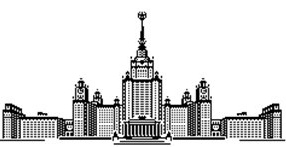
\includegraphics[width = 6cm, height = 4 cm]{msu.jpg}
			\label{fig:msu}
		\end{figure}
		\normalsize{{Московский  государственный
				университет имени М.В.~Ломоносова}}\\[0.1cm]
		\normalsize{{Факультет космических исследований}}\\[0.1 cm]
%   \normalsize{{Специальность 01.05.01 <<Фундаментальные математика и механика>>}}\\[0.1 cm]
% \normalsize{{ Образовательная программа <<Космические исследования и космонавтика>>}}
		\noindent\rule{16cm}{0.4pt}
		\vfill
	
		\hfill \break
		\textbf{\Large{Нейросетевые методы для декодирования тонкой моторики по биоэлектрической активности}}\\ [0.3cm]
        \normalsize{{Курсовая работа}}\\
		\vfill
		\normalsize
		\begin{flushright}
			Выполнил студент 3 курса группы 302\\
			Балановский Антон Леонидович\\[0.3cm]
			
			 
			
			Научный руководитель\\
			Доктор биологических наук,\\
            Профессор механико-математического факультета МГУ\\
            Лебедев Михаил Альбертович\\

			
		\end{flushright}
		\hfill \break
	\end{center}
	
	\vfill
	\begin{center}{Москва, 2025}\end{center}
	\thispagestyle{empty} 
	%\setlength{\headsep}{0.2in}\end{titlepage}
\end{titlepage}
\tableofcontents

\newpage

\section*{Введение}
\addcontentsline{toc}{section}{Введение}

В последние годы значительно возрос интерес к использованию биосигналов человека для управления техническими системами. Один из перспективных подходов -- применение сигналов электромиографии (ЭМГ) мышц руки в качестве интерфейса «человек--машина». Считывая электрическую активность мышц, можно расшифровать намерения или движения оператора и передать их на управляемое устройство. Потенциальные области применения подобных интерфейсов очень широки: от реабилитации пациентов и управления протезами конечностей до высокоточных систем дистанционного управления роботами и экзоскелетами. Например, уже показано, что интерфейс на основе ЭМГ способен генерировать непрерывные управляющие команды в трёхмерном пространстве на основе произвольной мышечной активности оператора \cite{1}. В экспериментах на параболических полётах было продемонстрировано, что даже в условиях невесомости точность работы такого ЭМГ-интерфейса практически не ухудшается (успешность выполнения задач ~89–96\% в различных положениях оператора) \cite{1, 2}. Это указывает на высокий потенциал применения ЭМГ-управления для дистанционного руководства робототехническими системами в космосе  
, например при внекорабельной деятельности или телероботике.

Не менее значимы и наземные применения подобных технологий, ЭМГ-сигналы могут использоваться в протезировании, так как по активности уцелевших мышц можно судить о задуманных движениях утраченной конечности и управлять моторизированным протезом руки или ноги. \cite{3,4} В клинической реабилитации пациентов после инсультов или травм методы ЭМГ - контроля применяются для управления роботизированными экзоскелетами и тренажёрами, помогая восстанавливать утраченные двигательные функции \cite{5}. В повседневной жизни интерфейсы, основанные на мышечных сигналах, рассматриваются как удобная альтернатива ручным контроллерам и голосовым командам, например, для управления инвалидными колясками, компьютерными устройствами или мобильными роботами \cite{6,7}.
Благодаря тому, что поверхностная ЭМГ регистрируется с помощью компактных носимых сенсоров, такой интерфейс может быть лёгким и ненавязчивым для пользователя, что особенно важно как для людей с ограниченными возможностями, так и для операторов в скафандрах, где применение привычных органов управления затруднено из-за громоздких перчаток и ограниченной подвижности.

Таким образом, технология декодирования поверхностных ЭМГ - сигналов в реальном времени открывает возможность создания новых естественных способов взаимодействия человека с машинами. Данная работа посвящена обзору современных методов машинного обучения, в частности нейронных сетей, применяемых для обработки и распознавания ЭМГ, а также исследованию их эффективности на конкретной задаче декодирования движений по сигналам мышц. В качестве примера рассматривается восстановление траекторий рукописного ввода (цифр) по ЭМГ-сигналам предплечья, что имеет применение как для бионических протезов и реабилитационных устройств, так и для перспективных интерфейсов ввода в условиях невесомости. Кроме того, описывается программно-аппаратный конвейер (pipeline) обработки ЭМГ в режиме реального времени – от сбора и фильтрации сигналов до их подачи в нейросетевую модель и формирования управляющих команд. 

\section{Обзор методов обработки ЭМГ}
Обработка сигналов ЭМГ традиционно включала этапы выделения признаков (статистических, частотных и др.) и последующую классификацию. Однако современное развитие глубокого обучения позволяет осуществлять «конец-в-конец» декодирование, непосредственно извлекая нужную информацию из сырых многомерных сигналов без ручного формирования признаков \cite{8}. Ниже рассмотрены основные типы нейронных сетей, которые нашли применение в задачах распознавания по ЭМГ: сверточные, рекуррентные (в том числе сети долгой краткосрочной памяти LSTM) и трансформеры.

\subsection{Сверточные нейронные сети (CNN)}
CNN успешно применяются и к временным рядам, включая ЭМГ-сигналы. Это позволяет автоматически фильтровать и усиливать информативные особенности мышечных сигналов – например, характерные формы активации, спектральные компоненты и т.д. – без явного задания признаков экспертом \cite{9}. В работах последних лет показано, что глубокие CNN способны превосходить по точности традиционные классификаторы на основе вручную отобранных признаков \cite{10}. Так, первое применение CNN для распознавания жестов по ЭМГ (Atzori et al., 2016) продемонстрировало качество, сопоставимое с классическими методами на том же наборе данных \cite{11}. Более сложные архитектуры, такие как многопоточная сверточная сеть (MSCNN), позволили улучшить результат за счёт одновременного анализа сигналов с нескольких мышц \cite{12}. В частности, Wei et al. (2019) предложили объединять несколько сверточных потоков, обучающихся на разных группах каналов ЭМГ, и добились более высокой точности по сравнению с одиночной CNN и случайным лесом \cite{13}. Однако увеличение числа каналов и потоков приводит к росту вычислительной сложности модели \cite{14}. В практических приложениях это требует баланса между точностью и быстродействием.


CNN хорошо зарекомендовали себя в задачах классификации дискретных состояний или жестов по ЭМГ. Например, в работе Ameri et al. (2018) предложена система управления протезом на основе CNN, которая в реальном времени различает несколько одновременно выполняемых движений кисти \cite{15}. Сверточная сеть, аналогичная по архитектуре классическим моделям компьютерного зрения (например, AlexNet), была обучена сопоставлять многоканальные ЭМГ-сигналы различным комбинациям движений запястья \cite{16}. Отмечается, что такая CNN-модель способна автоматически выучивать эффективные признаки (вместо ручного расчёта статистик сигналов) и благодаря этому обеспечивать более плавное и точное управление искусственной конечностью \cite{15}. Ещё одним направлением является применение предобученных CNN, перенастроенных под ЭМГ-данные (transfer learning). В недавнем исследовании для классификации эмоций по ЭМГ предплечья использовали спектрограммы сигналов в качестве входных «изображений» и предобученные сети AlexNet, GoogleNet, ResNet, добившись высокой точности распознавания \cite{17}. Эти примеры подтверждают, что сверточные нейросети эффективно выделяют структурные особенности мышечных сигналов и могут служить ядром ЭМГ-интерфейсов различного назначения.



\subsection{Рекуррентные нейронные сети (RNN)}
 RNN принципиально отличаются от CNN способностью обрабатывать последовательности произвольной длины, благодаря наличию обратных связей. Главное преимущество RNN – учёт временной динамики: сеть обучается напрямую находить закономерности во временной структуре сигналов, минуя стадию сегментации на независимые окна. В результате RNN могут извлекать из EMG-фрагмента все детали, важные для классификации или регрессии, не теряя информацию при усреднении по окну \cite{18}. Более того, рекуррентная сеть может работать напрямую с сырым сигналом, что исключает этап ручного конструирования признаков и упрощает предобработку данных \cite{19}. Исследования показывают высокую эффективность такого подхода. Например, Alvarez-Alvarado et al. (2024) протестировали несколько RNN-архитектур (включая LSTM, GRU и двунаправленную сеть) на задаче классификации 5 движений руки по ЭМГ и получили точность ~98\%, значительно превышающую результат SVM (~93\%) \cite{20}. При этом LSTM-сеть не только была точнее классического метода, но и обеспечила самую быструю классификацию – порядка 0.12 мс на образец \cite{20}, что важно для реального времени.

Однако у рекуррентных сетей есть и недостатки. Из-за последовательной природы вычислений RNN сложнее распараллеливать, поэтому обучение и предсказание могут занимать больше времени по сравнению с сверточными сетями, особенно на длинных последовательностях \cite{21}. Кроме того, со временем точность RNN-моделей на продолжительных записях может снижаться, если сеть не обладает достаточной памятью или не обучена учитывать медленные изменения статистики сигнала \cite{22}. Для повышения устойчивости во времени исследователи пробуют увеличивать глубину и размер рекуррентных сетей, но это чревато переобучением и ещё большим замедлением обучения \cite{23}. В связи с этим в ряде работ применяются гибридные подходы: например, сети, сочетающие сверточные и рекуррентные слои. CNN в такой связке берёт на себя извлечение локальных признаков ЭМГ, а RNN обрабатывает последовательность этих признаков во времени, сохраняя контекст \cite{24}. Показано, что подобные гибриды могут обучаться эффективнее, чем «чистые» RNN, и давать более высокую точность на динамических жестах \cite{25}. В частности, CNN-LSTM модель классификации 6 движений голеностопа превзошла по точности отдельно CNN и отдельно LSTM, достигнув 95.7\% верных распознаваний \cite{26}.


\subsection{Сети долгой краткосрочной памяти (LSTM)}
**Сети долгой краткосрочной памяти (LSTM).** 

Сети LSTM (Long Short-Term Memory) представляют собой усовершенствованный вариант рекуррентных сетей, специально разработанный для хранения долговременной информации. В узлах LSTM введены так называемые «элементы памяти» (memory cells) с механизмом трёх шлюзов (gate): входного, выходного и «затвора забывания». Благодаря этим шлюзам LSTM самостоятельно регулирует, какую часть информации из потока сигналов сохранить в памяти, а какую стереть как несущественную. Такая архитектура позволяет учиться на более длительных последовательностях. Для анализа ЭМГ LSTM особенно ценна, поскольку может удерживать в скрытом состоянии признаки начальных фаз движения вплоть до его завершения, что улучшает целостность распознавания сложных многоскоростных или многоэтапных действий.

Практический опыт показывает, что LSTM в большинстве случаев превосходит классические RNN на задачах классификации ЭМГ. Например, в упомянутой работе Alvarez-Alvarado (2024) LSTM-сеть дала наивысшую точность (98.5\%) и скорость классификации среди всех протестированных моделей(GRU, Bidirectional RNN, SVM) \cite{20}.  Другие исследования подтверждают, что LSTM устойчивее к шумам и пропускам сигналов при реальной работе интерфейса по сравнению с простыми рекуррентными узлами. Ещё одно преимущество LSTM – гибкость: эти сети легко модифицируются под задачу, например, могут быть двунаправленными (BiLSTM) для учёта контекста с двух сторон, либо объединяться с сверточными слоями. 

Тем не менее, LSTM остаются вычислительно более сложными, чем однослойные CNN, и требуют тщательной настройки гиперпараметров. При большом количестве нейронов и длинных последовательностях время обучения LSTM существенно возрастает, а параллельное выполнение ограничено. Кроме того, для хорошей обобщающей способности LSTM обычно нужны более объёмные датасеты, чем для CNN, чтобы сеть могла корректно настроить свои многочисленные параметры памяти. В случае недостатка данных может наблюдаться переобучение на конкретных траекториях сигналов.

\subsection{Трансформеры}
Трансформер (Transformer) – один из новейших типов нейросетевой архитектуры, который за последние годы совершил революцию в обработке последовательностей, прежде всего в области естественного языка. Главное отличие трансформера от RNN – использование механизма self-attention вместо рекуррентных связей. Это позволяет трансформеру параллельно обрабатывать весь входной последовательный сигнал, взвешивая взаимное влияние разных его элементов. Сеть на основе трансформеров способна эффективно улавливать дальние связи внутри данных и строить представление всего временного ряда как единого контекста \cite{27}. При этом, в отличие от RNN, время обучения не растёт линейно с длиной последовательности благодаря возможности параллелизации вычислений самовнимания \cite{28}.
Изначально трансформеры получили наибольшее распространение в задачах NLP и машинного перевода, однако постепенно их начали применять и в обработке биосигналов (ЭЭГ, ЭМГ и др.) \cite{29}. В области распознавания жестов по многоканальным ЭМГ уже появились работы, демонстрирующие конкурентоспособность трансформерных моделей. Так, Rahimian et al. (2021) предложили архитектуру на основе Vision Transformer (ViT) для классификации 17 жестов кисти (датасет NinaPro DB2) и достигли точности, сопоставимой с лучшими на тот момент методами глубокого обучения \cite{30}. Montazerin et al. (2022) адаптировали визуальный трансформер для задачи идентификации жестов по высокоплотной ЭМГ (128-канальный массив электродов) и также получили превосходные результаты \cite{31}. Эти исследования подтверждают, что трансформер способен эффективно извлекать временные и пространственные характеристики активности мышц и добиваться высокой точности распознавания \cite{32}.
Важно отметить, что трансформерные модели, хотя и обладают большой мощностью, предъявляют высокие требования к объёму данных для обучения. В отличие от CNN, которые в своей архитектуре «вшивают» априорные допущения о локальности и смещении признаков, трансформер изначально не имеет подобных ограничений \cite{33}. Это означает, что для успешного обучения ему требуется больше обучающих примеров, чтобы самостоятельно выявить все полезные зависимости. При малом датасете трансформер может переобучиться или найти неустойчивые решения. Кроме того, самовнимание имеет квадратичную сложность по длине последовательности, поэтому очень длинные сигналы обрабатывать тяжело по ресурсам. В экспериментальных системах по распознаванию жестов трансформеры пока часто используют подходы, заимствованные из обработки изображений (представляя многоканальный сигнал в виде «картинки» или набора патчей), и не всегда учитывают специфические особенности ЭМГ \cite{34}. Тем не менее, архитектуры на базе трансформера сейчас являются предметом активных исследований в сфере биомедицинских сигналов, и ожидается, что с накоплением больших массивов данных они смогут установить новый стандарт качества распознавания.

\subsection*{Переход к конкретной задаче: распознавание рукописных символов по ЭМГ}
\addcontentsline{toc}{subsection}{Переход к конкретной задаче: распознавание рукописных символов по ЭМГ}
После обзора общих подходов перейдём к частному примеру задачи декодирования движений руки по ЭМГ, который будет рассматриваться в практической части работы. Речь идёт о распознавании рукописных цифр и восстановлении траекторий «почерка» по сигналам поверхностной ЭМГ предплечья. Данная задача впервые была решена 2009 \cite{35}, где авторы показали принципиальную осуществимость реконструкции написанного текста только на основании мышечной активности.В их эксперименте испытуемые выводили цифры от 0 до 9 ручкой на дигитайзере, одновременно с этим с восьми электродов, размещённых на предплечье и кисти, регистрировалась ЭМГ. Был разработан алгоритм, который сначала восстанавливал траекторию движения ручки (координаты X–Y во времени) по сигналам ЭМГ, а затем определял, какая цифра написана, методом шаблонного распознавания. Несмотря на то, что применённые методы были относительно простыми (линейная регрессия и линейный дискриминантный анализ), результаты оказались обнадеживающими. Средняя точность автоматического распознавания цифр достигла ~90\% при использовании всех 8 каналов ЭМГ\cite{35}, а восстановленные компьютерным алгоритмом траектории рукописи по форме близко совпадали с реальными (коэффициент детерминации $R^2 \approx 0.5$–$0.6$ между восстановленными и истинными координатами). По сути, это доказало, что поверхность руки генерирует достаточно информативные электрические сигналы, способные «кодировать» сложные мелкомоторные движения (такие как письмо или рисование), и эти сигналы можно расшифровать программно.

Важно подчеркнуть, что в статье. для решения задачи письма по ЭМГ были использованы не нейросети, а классические алгоритмы: так называемый фильтр Винера (Wiener filter) для реконструкции координат и линейный дискриминантный анализ (ЛДА) для классификации символов. Фильтр Винера представлял собой линейную модель, вычисляющую каждую координату $(x(t), y(t))$ кончика ручки как взвешенную сумму значений ЭМГ на всех каналах за небольшой интервал времени до момента\cite{36, 37}. Коэффициенты (веса) этой модели подбирались методом наименьших квадратов по тренировочным записям “почерка” и соответствующих ЭМГ. При последующем применении модели к новым сигналам она формировала траекторию пера без участия человека. Несмотря на линейность такого подхода, он вполне успешно восстановил общую форму написанных цифр. Для опознания самой цифры (чтобы, например, распечатать ее символом) использовался ЛДА: сегменты ЭМГ, соответствующие написанию каждого символа, сравнивались с шаблонами от каждого из 10 символов, и выбирался класс с наибольшим сходством. В этой части задача эквивалентна многоклассовой классификации временных рядов. Достигнутая точность ~90\% означает, что в большинстве случаев цифры удавалось различить правильно, хотя и наблюдались ошибки между схожими по написанию символами (например, «3» и «8»). 

Исследование Linderman et al. является отправной точкой для нашей работы, поскольку предоставило открытый набор данных ЭМГ и траекторий (см. следующий раздел) и базовый уровень качества декодирования, с которым можно сравнивать современные методы на основе нейросетей. Ожидается, что применение глубинных нейронных сетей (CNN, LSTM и др.) позволит улучшить как точность распознавания рукописных символов, так и степень приближения восстановленной траектории к реальной. Кроме того, такой подход будет более универсальным: обученная сеть сможет адаптироваться и к другим видам движений (не только письму), что важно для создания многофункциональных интерфейсов на основе ЭМГ.

\section{Выбор и характеристика датасета}
Для экспериментальной части работы выбран датасет, опубликованный в статье Recognition of Handwriting from Electromyography  в журнале PLOS ONE \cite{35}. Этот набор данных содержит синхронные записи ЭМГ и траекторий движения пера при письме цифр, полученные от группы здоровых добровольцев. Всего в эксперименте участвовало 6 человек. Каждый испытуемый писал стандартным почерком цифры от «0» до «9» в специальном окне на планшете. Для каждой цифры выполнялось 50 повторных написаний (итого 500 символов на участника). Во время письма с поверхности руки и предплечья регистрировались 8-канальные ЭМГ-сигналы: использовались поверхностные электроды, наложенные на основные мышцы, управляющие пальцами и кистью. Частота дискретизации ЭМГ и координат составляла 1000~Гц, сигналы ЭМГ предварительно полноволново детектировались и фильтровались (сглаживались) фильтром низких частот 5~Гц, чтобы выделить огибающую мышечной активности. Для каждого написанного символа в датасете сохранены: временной ряд координат $x(t)$ и $y(t)$ траектории ручки, а также 8 временных рядов ЭМГ (по числу каналов) за интервал времени написания (около 2--3 секунд).

Данный датасет подходит для целей нашей работы по нескольким причинам. Во-первых, он является открытым и общедоступным, что упрощает воспроизводимость экспериментов. Во-вторых, структура данных идеально соответствует поставленной задаче: присутствуют как непрерывные данные (траектории движений), так и дискретные метки классов (цифры), связанные с записями ЭМГ. Это позволяет проверять и регрессионные подходы (восстановление сигналов управления в реальном времени), и методы классификации (распознавание команд или жестов). В-третьих, набор достаточно велик (6 субъектов, суммарно 3000 примеров символов) для обучения современных нейросетевых моделей, но при этом относительно компактен по объёму, что даёт возможность проводить эксперименты без чрезмерных вычислительных затрат. В-четвёртых, данные получены в контролируемых лабораторных условиях с жёсткой фиксацией задачи (фиксированный набор символов, ограниченная область письма, постоянное положение электродов в течение сессии), что снижает вариабельность и шум, не связанные с целью эксперимента.
Наконец, следует отметить, что рассматриваемый датасет представляет интерес с точки зрения потенциальных космических применений. Письмо или рисование – это тонкая моторика, требующая координированной работы многих мышц руки. Если удаётся успешно декодировать именно такие движения, то можно ожидать, что более крупные жесты (нажатия кнопок, сгибание пальцев, хватательные движения), которые могут понадобиться астронавту в скафандре для управления робототехникой, тем более будут различимы по ЭМГ. Таким образом, эти данные служат хорошей «проверочной площадкой» для нейросетевых алгоритмов декодирования: на них можно отработать подходы, а затем перенести их на другие сценарии (например, управление манипулятором или беспилотным аппаратом по ЭМГ-сигналам оператора).

\section{Иллюстрации и анализ данных}
Для наглядного представления исходных данных и результатов декодирования приведём несколько иллюстраций из проведённых экспериментов. 

\begin{figure}[h]
\centering
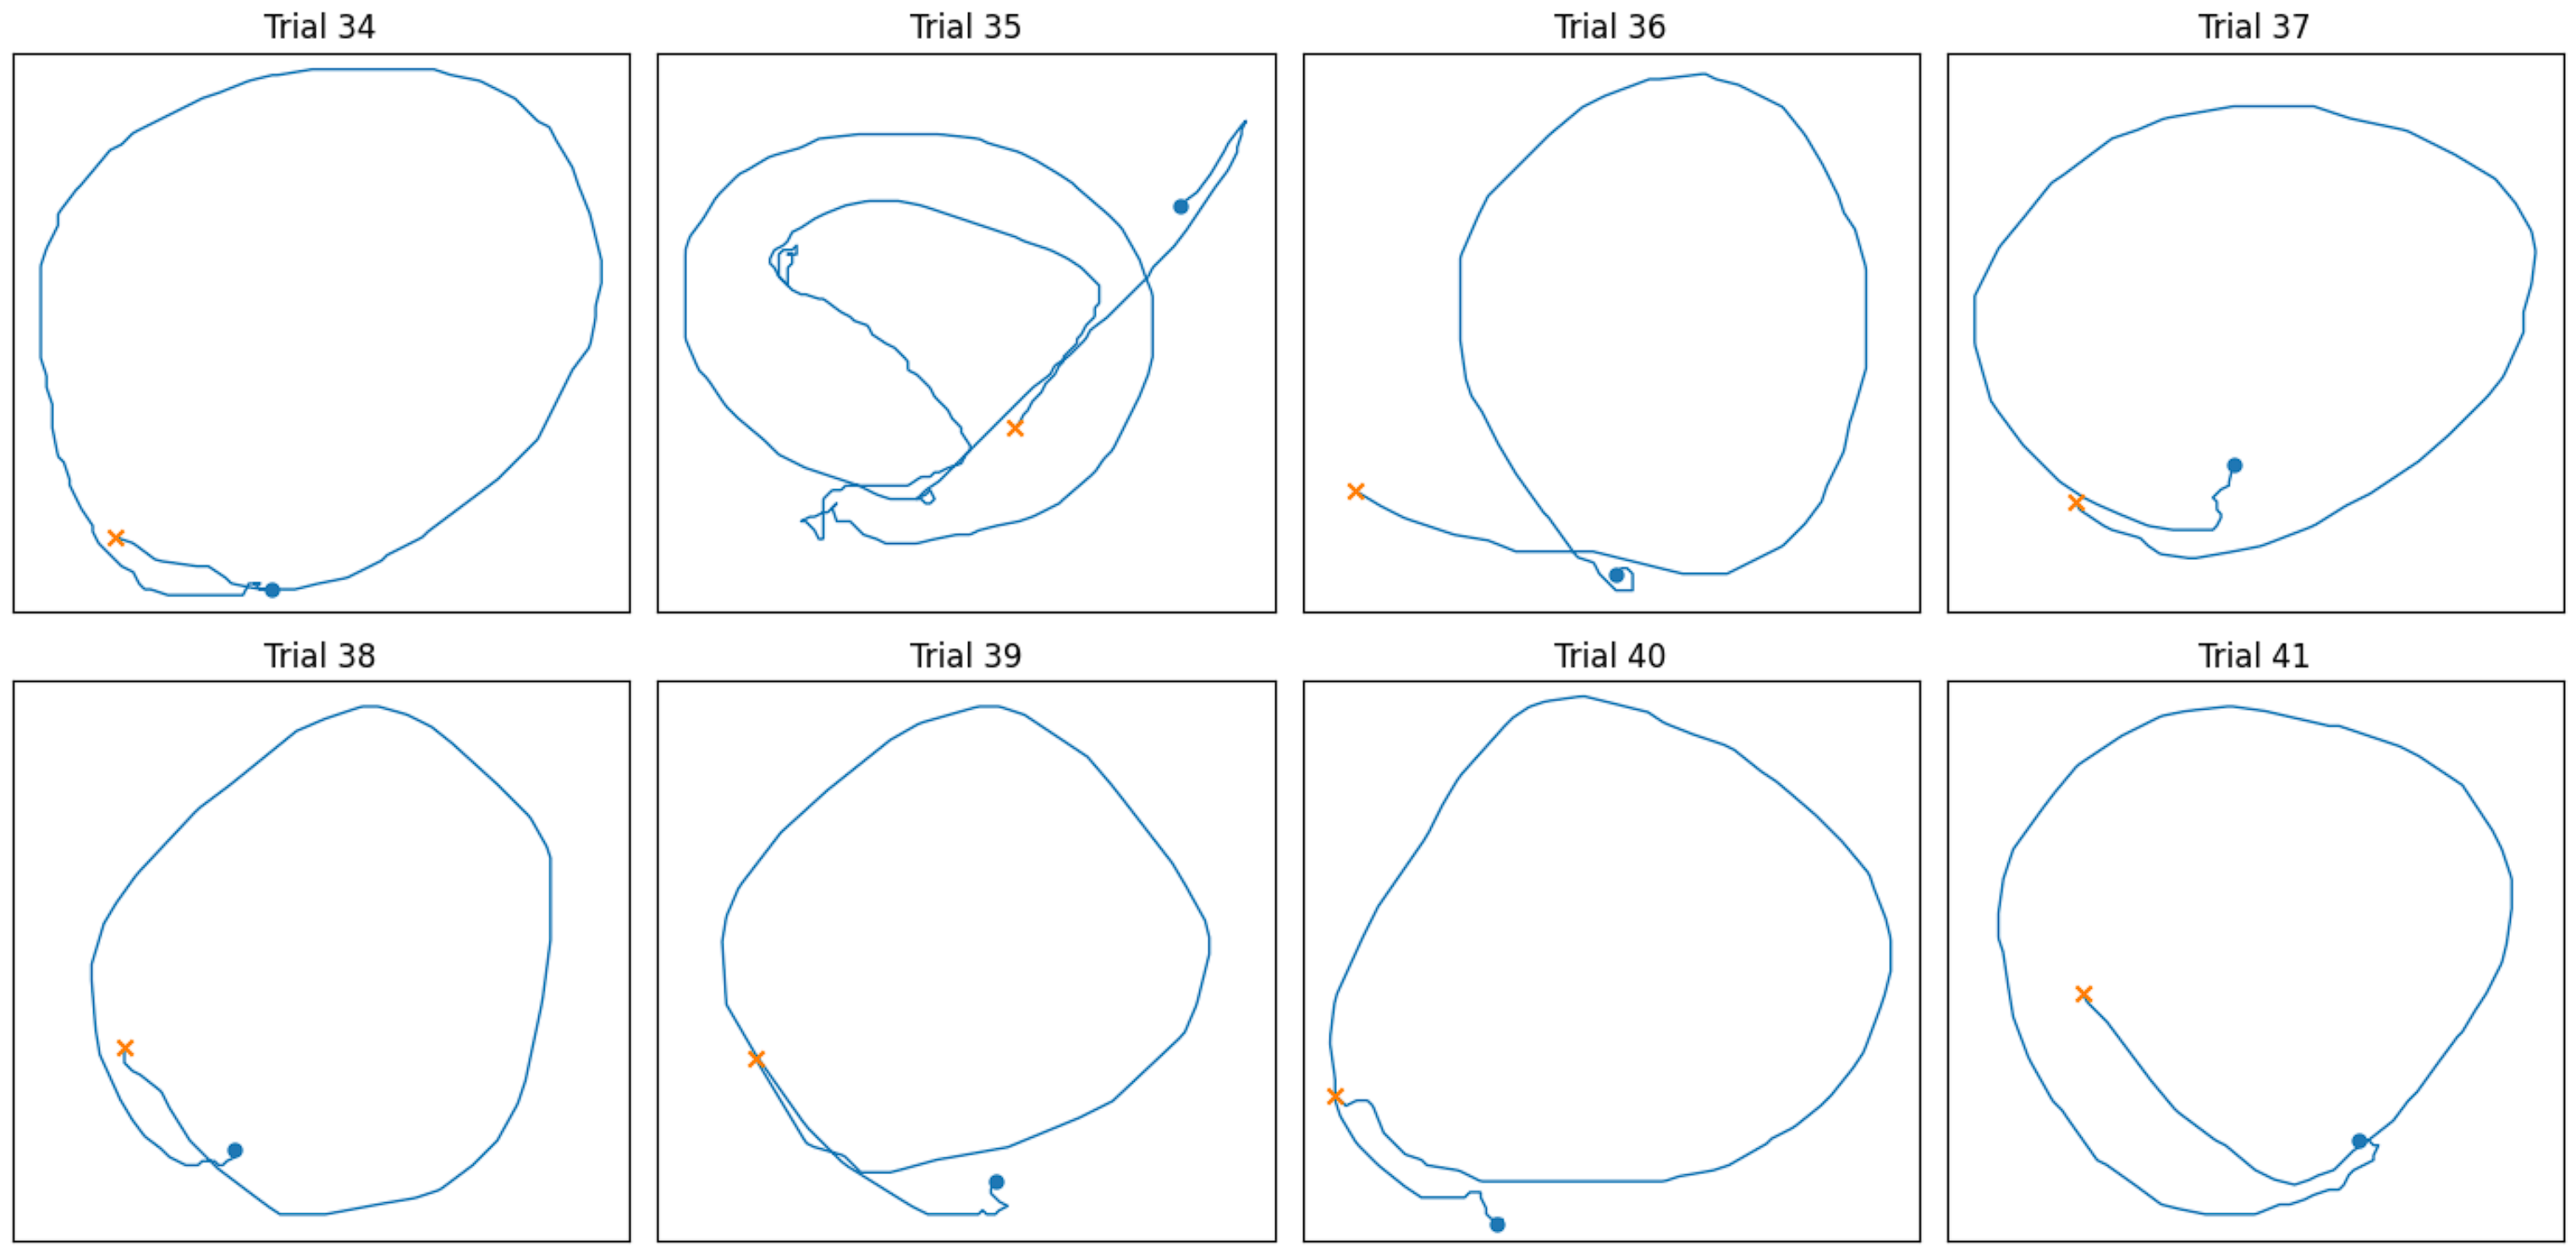
\includegraphics[width=0.95\textwidth]{img1.png}
\caption{оригинальные траектории для нескольких попыток (Trial 34--41).}
\label{fig:traj}
\end{figure}

На рис.~\ref{fig:traj} показаны оригинальные координаты пера, напрямую считанные с графического планшета в эксперименте,\cite{35}. Каждая синяя линия соответствует одной попытке написания цифры «0» (сеансы 34–41); оранжевый крестик — точка начала штриха, синий кружок — точка окончания.

Несмотря на то, что все восьмерки образуют замкнутый «нуль», траектории различаются по радиусу, смещению и ориентации — естественная вариабельность моторики человека. Поэтому датасет ценен двойным образом:

Классификация: по разметке XY можно однозначно назвать символ, что даёт точную целевую метку для обучения распознавания цифр по ЭМГ.

Декодирование движения: имея согласованные пары «ЭМГ → координаты пера», можно обучать модели прямого предсказания текущего направления и скорости руки, т.е. решать задачу непрерывного моторного управления.

\begin{figure}[h]
\centering
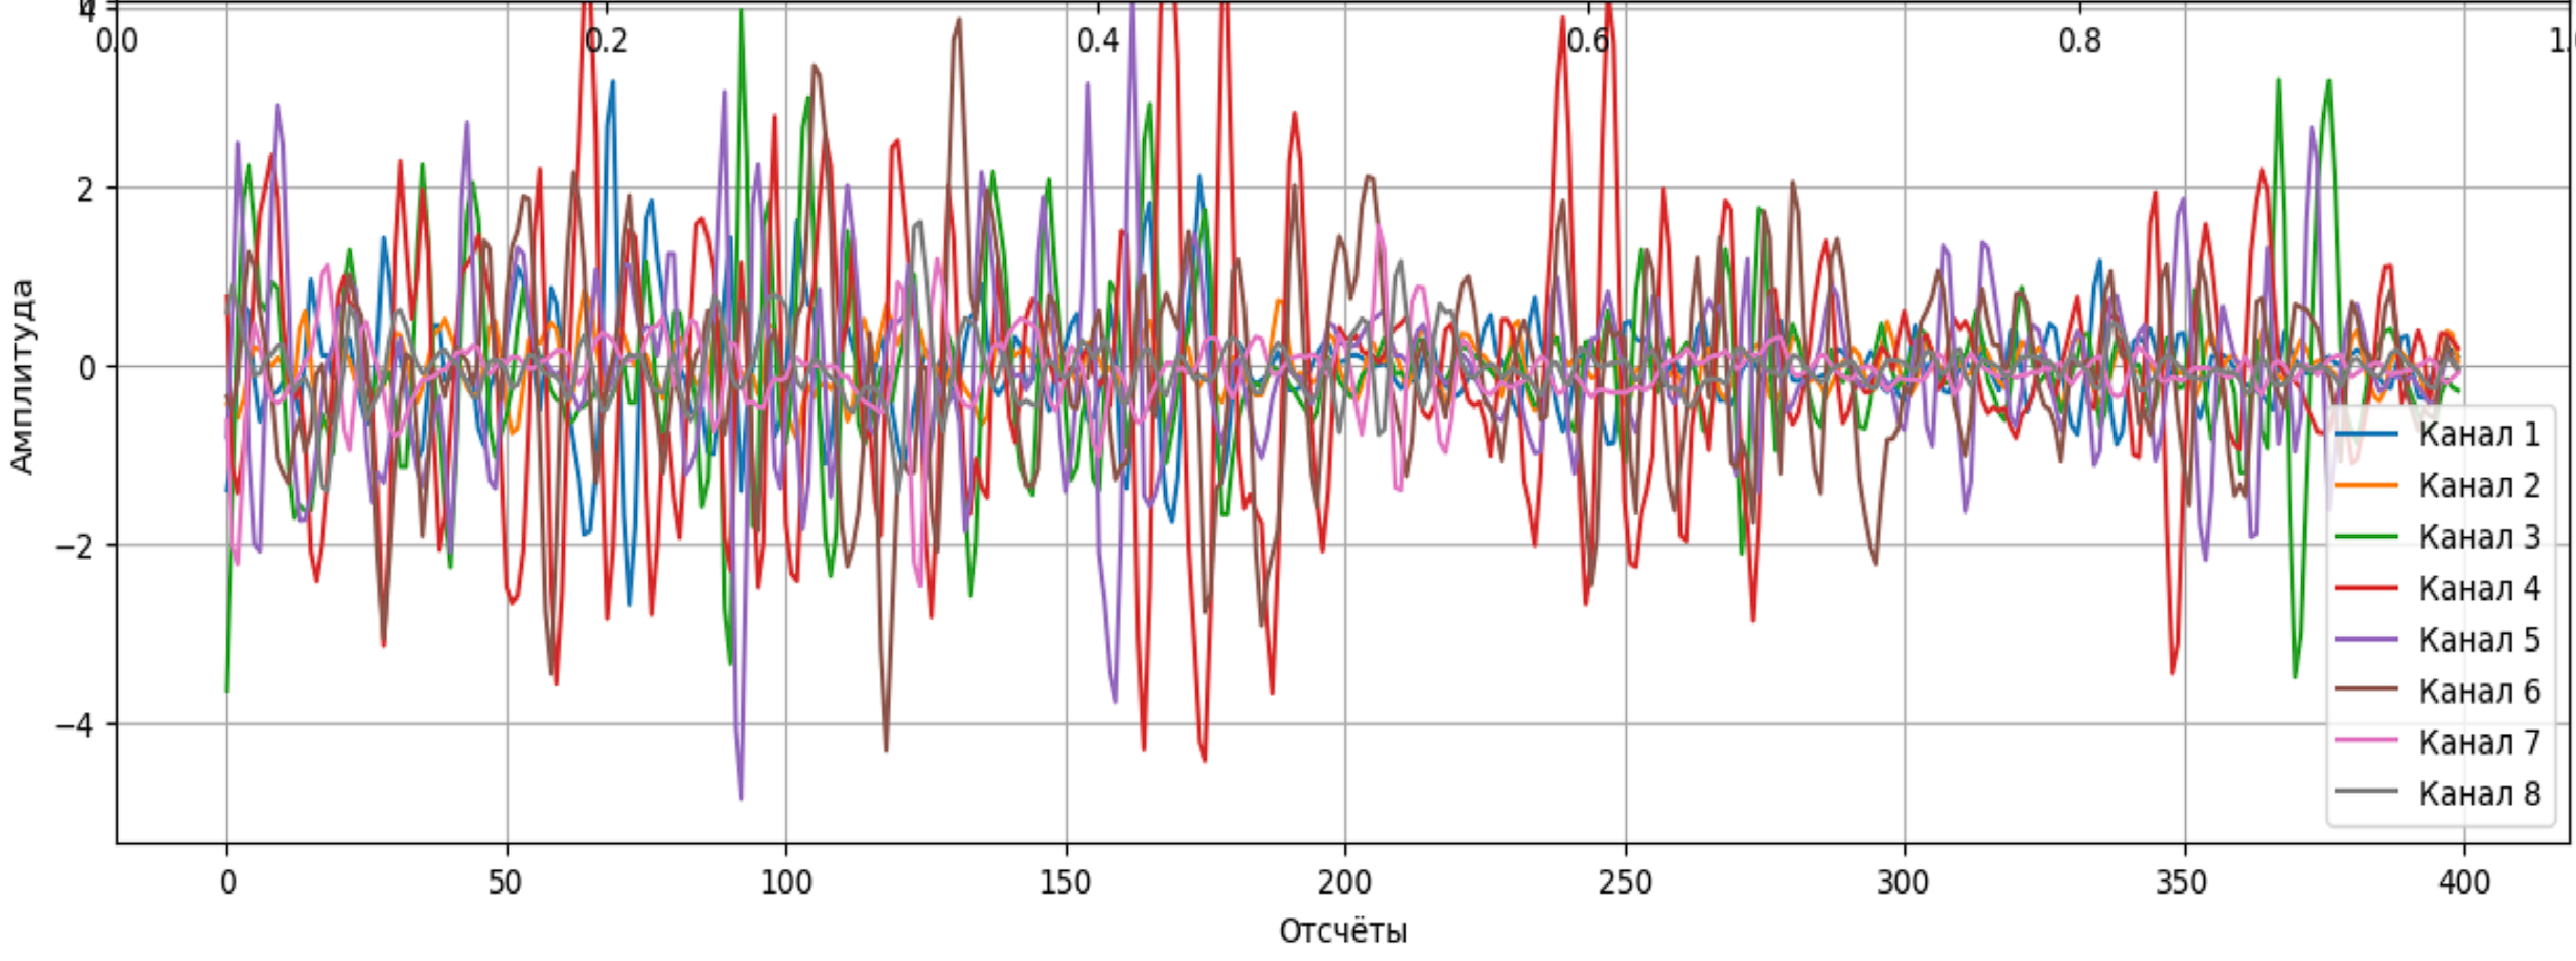
\includegraphics[width=0.9\textwidth]{img2.png}
\caption{Сырые сигналы восьми каналов ЭМГ во время выполнения одного движения (написание символа). Видно, что различные мышцы (каналы) активируются с разной амплитудой и в разные моменты времени, формируя характерный «почерк» сигнала для данного жеста.}
\label{fig:raw_emg}
\end{figure}

На рис.~\ref{fig:raw_emg} приведён пример сырых ЭМГ-сигналов со всех 8 каналов, зарегистрированных при написании одного символа (вертикальная ось – амплитуда, горизонтальная – время, отложенное в условных отсчётах). Каждый цветной график соответствует отдельному каналу (электроду), размещённому над определённой мышцей предплечья или кисти. Можно заметить, что во время движения разные мышцы проявляют различную активность: например, канал~4 (красная кривая) имеет выраженные всплески амплитуды примерно в середине и конце движения, канал~2 (оранжевый) показывает особенно сильный выброс ближе к 0.6~с, а некоторые другие каналы колеблются менее явно. Такая картина отражает биомеханику написания конкретной цифры: одни мышцы напрягаются сильнее при выводе определённых элементов траектории, тогда как другие остаются относительно пассивными. По совокупности сигналов всех каналов можно однозначно идентифицировать движение – фактически, эта многомерная временная запись и есть «мышечный почерк», индивидуальный для каждого символа. Однако визуально интерпретировать эти графики человеку затруднительно. Задача алгоритма распознавания (нейросети) – выявить скрытые закономерности в этих 8-канальных временных сериях и сопоставить их либо определённой цифре (для классификации), либо конкретной координатной траектории (для регрессии). 

Прежде чем подавать данные в модель, обычно производится ряд этапов предварительной обработки. На приведённом рисунке показаны уже отфильтрованные сигналы, чтобы продемонстрировать общий вид ЭМГ. В пайплайне, обычно, сырые записи проходят через фильтры, удаляющие низкочастотный дрейф и сетевые наводки, затем нормализуются по амплитуде, и из них выделяются короткие сегменты (окна), в пределах которых анализируется частотный состав. Ценность информации заключена не столько в мгновенных значениях ЭМГ (которые хаотичны), сколько в их статистических характеристиках – энергии сигнала, спектре частот, числе активных всплесков за интервал и т.д.

\begin{figure}[h]
\centering
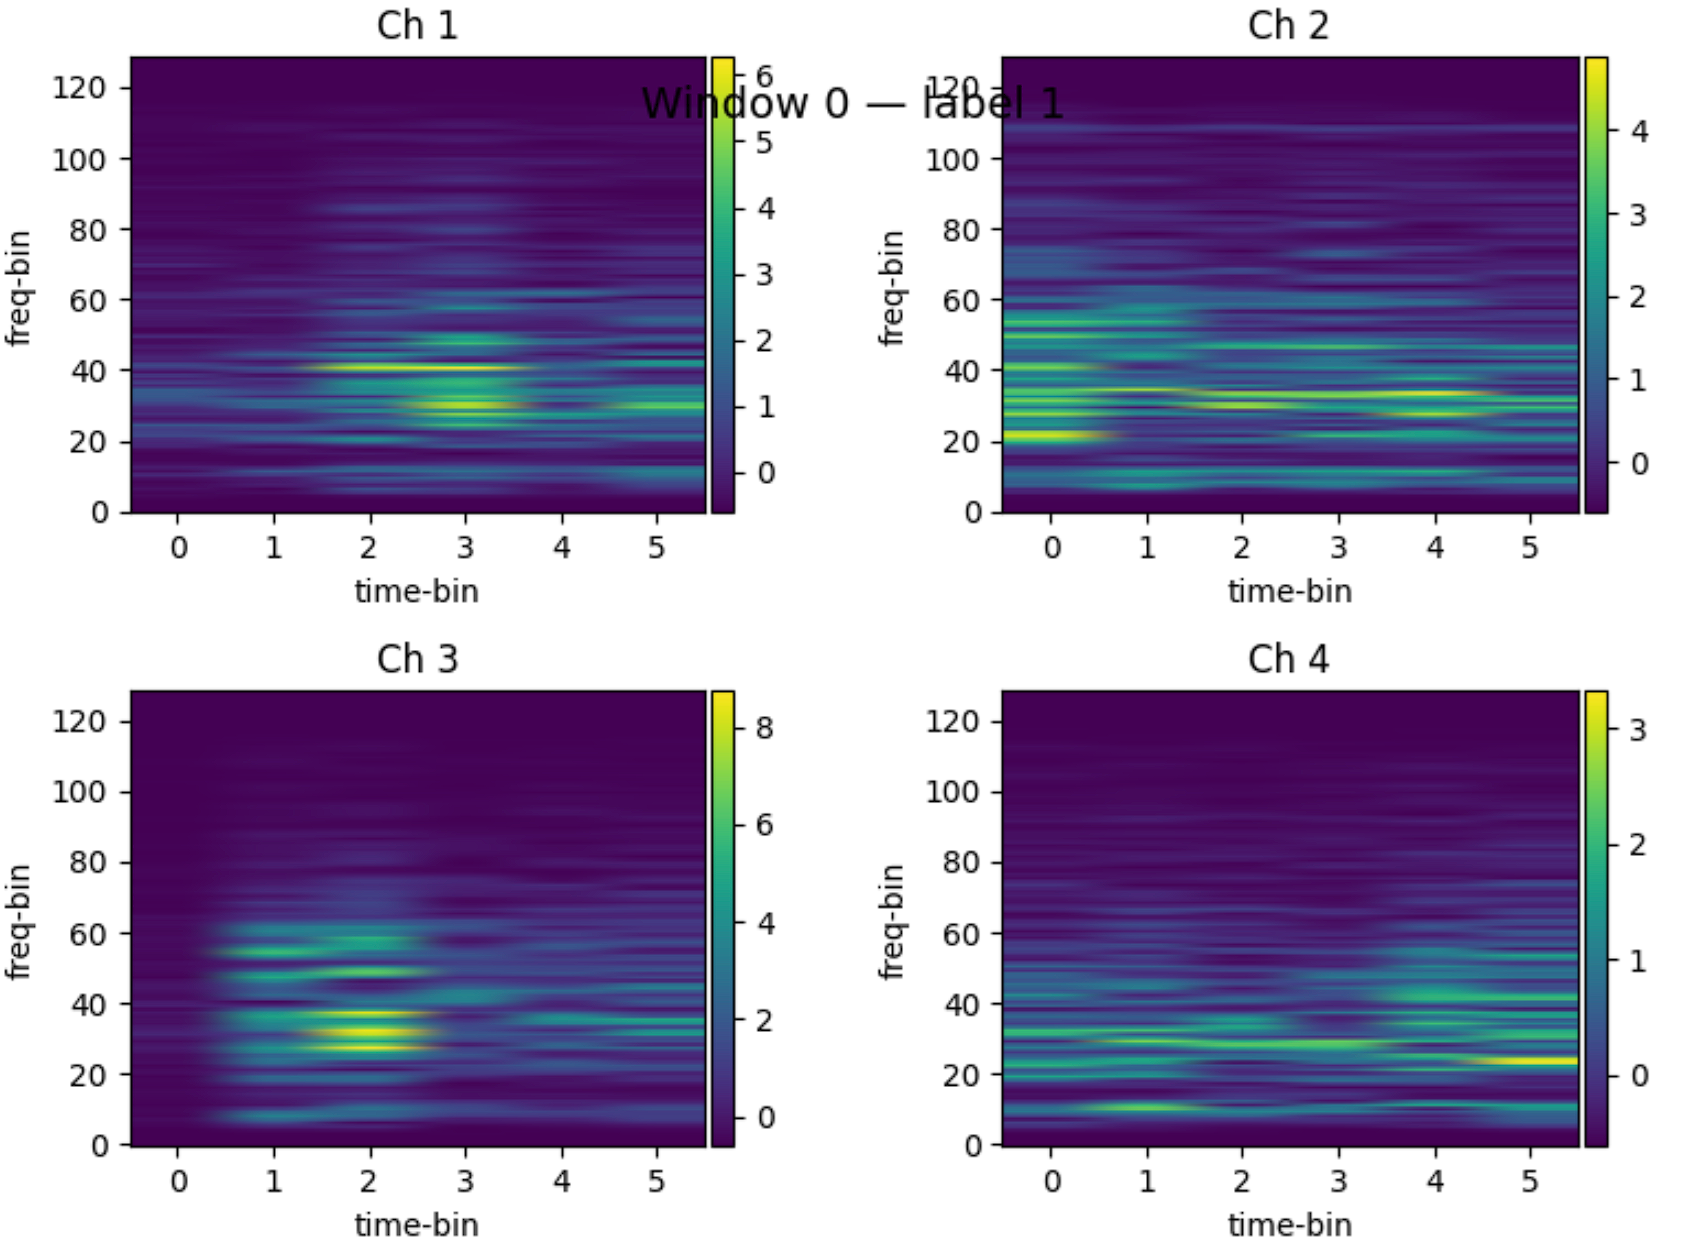
\includegraphics[width=0.8\textwidth]{img3.png}
\caption{Спектрограммы (временные частотные характеристики) сигналов ЭМГ на каналах 1--4 за один фрагмент движения (длительностью около 5~с). По горизонтали отложено время (разбиение на окна), по вертикали – номер частотного диапазона, цветом показана мощность сигнала в соответствующей полосе частот.}
\label{fig:spectrogram1}
\end{figure}

\begin{figure}[h]
\centering
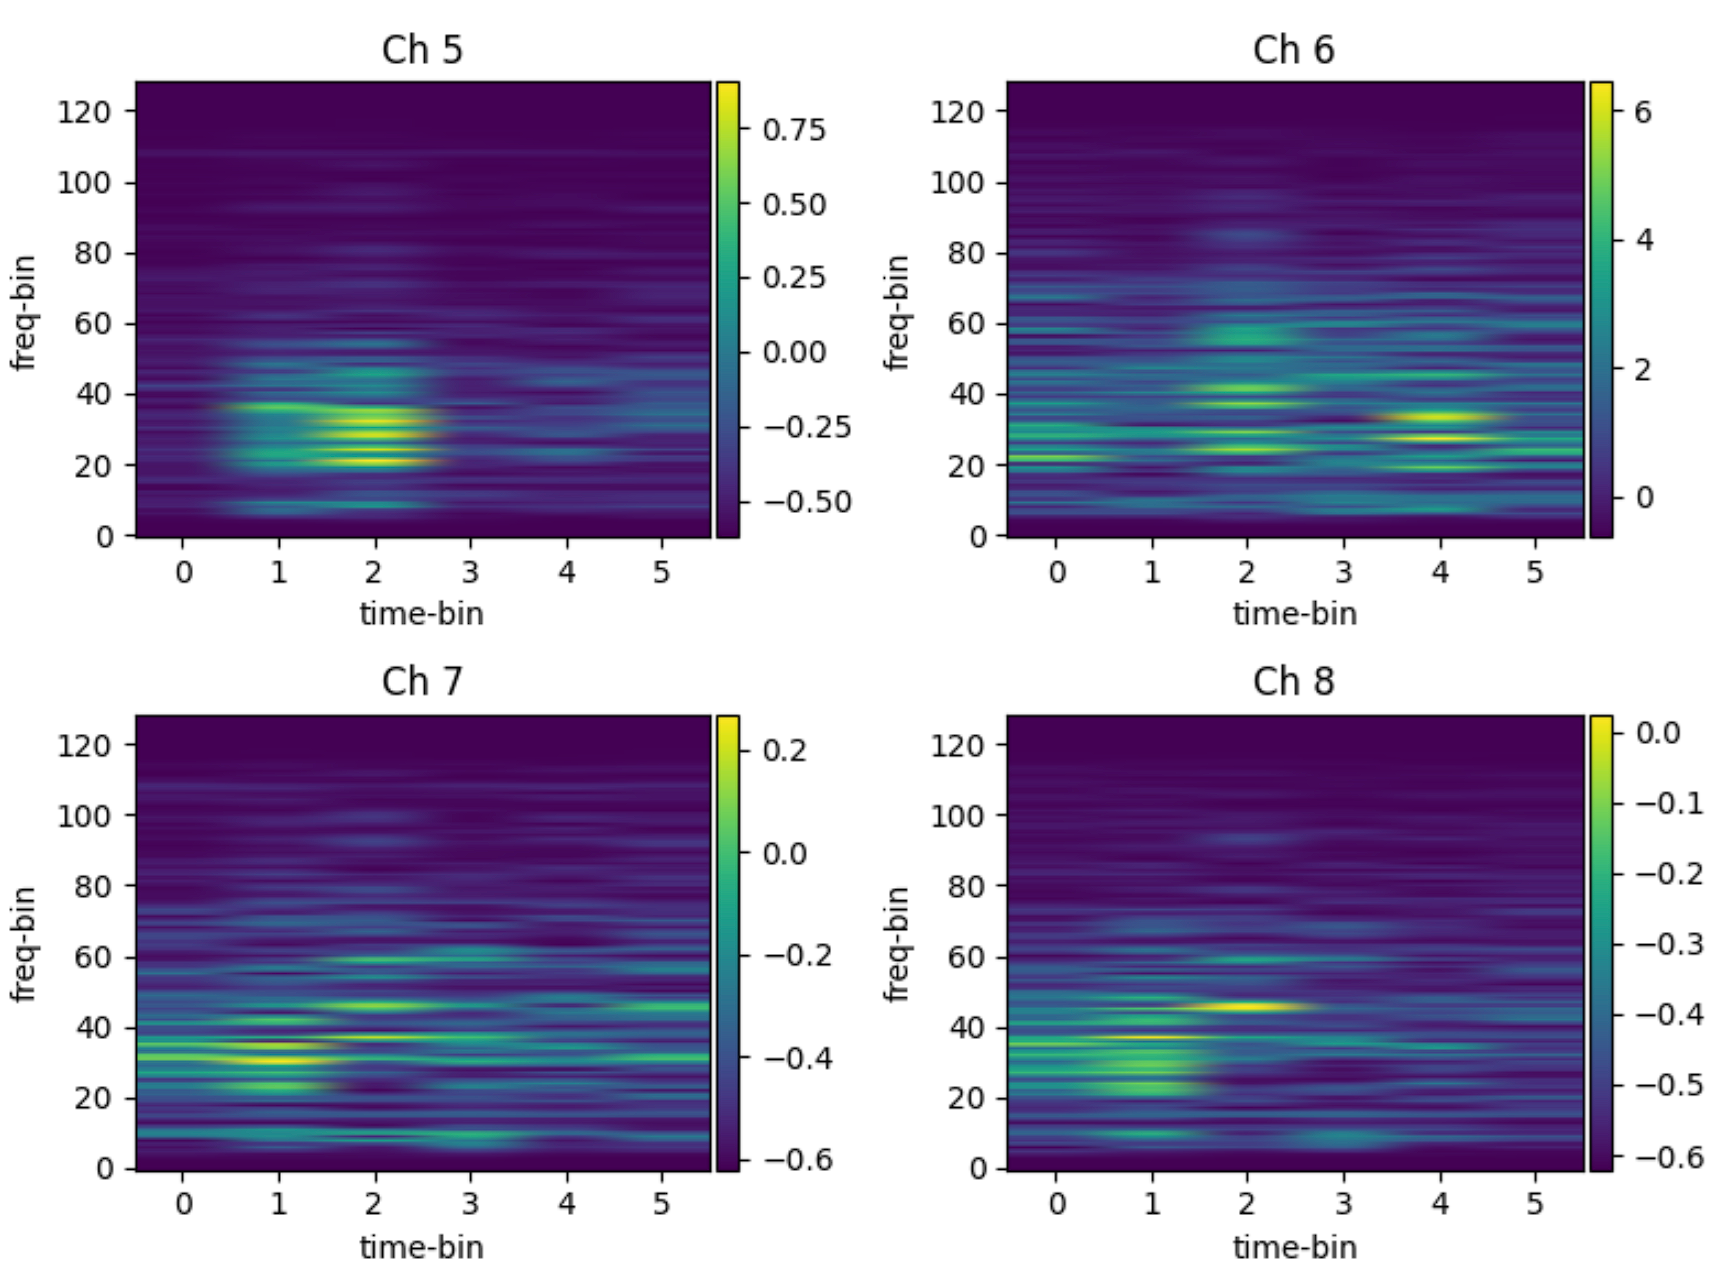
\includegraphics[width=0.8\textwidth]{img4.png}
\caption{Спектрограммы сигналов на каналах 5--8 для того же временного фрагмента, что и на рис.~\ref{fig:spectrogram1}. Видно, что распределение мощности по частотам отличается для разных мышц, отражая их вклад в движение.}
\label{fig:spectrogram2}
\end{figure}

Рисунки~\ref{fig:spectrogram1} и \ref{fig:spectrogram2} иллюстрируют спектральное представление тех же сигналов ЭМГ. Здесь показаны спектрограммы для каналов~1--4 и 5--8 соответственно, полученные разбиением сигналов на короткие окна и вычислением мощности в наборе частотных полос внутри каждого окна с помощью быстрого Фурье-преобразования. По оси времени отложены индексы окон (0--5 на рисунке соответствуют времени порядка 0--0.5~с), по оси частоты – порядковые номера полос. Интенсивность цвета (от фиолетового к жёлтому) показывает величину спектральной плотности мощности ЭМГ в данной полосе на данном интервале времени. Спектрограммы наглядно демонстрируют, как меняется частотная структура мышечных сигналов в процессе движения. Можно заметить, что на некоторых каналах (например, Ch~3 на рис.~\ref{fig:spectrogram1}) в середине записи появляется яркая зона в диапазоне около 40 – это означает всплеск активности определённой мышцы, выраженный в росте энергии сигналов на этих частотах. В других каналах, напротив, картина более равномерна (например, Ch~4 на рис.~\ref{fig:spectrogram1} показывает относительно невысокую мощность на всех частотах). Сопоставление спектрограмм различных каналов подтверждает, что каждый из 8 сигналов несёт уникальную информацию о движении, а их комбинация даёт полную картину. Для алгоритмов машинного обучения спектрограмма является удобным входным представлением, поскольку преобразует исходный одномерный сигнал в двумерное «изображение», где скрытые признаки могут быть выделены теми же методами, что и в компьютерном зрении (например, с помощью сверточных фильтров CNN). В данном проекте именно спектральные «карты» ЭМГ используются в качестве входных данных для нейронной сети, о чём подробнее рассказано далее.

\section{Конвейер обработки сигналов в реальном времени}
Разработка интерфейса управления роботами на основе ЭМГ требует создания цепочки программно-аппаратных модулей, обеспечивающих непрерывный съём, обработку и декодирование сигналов с минимальной задержкой.

\subsection{Два минимальных конвейера обработки}

% ---------- PIPELINE A ----------
\paragraph{Pipeline A: «CNN-Lite» (быстрый базовый).}
\begin{enumerate}
  \item \textbf{Фильтрация} — notch 50 Гц $\to$ Band-pass 20–450 Гц.
  \item \textbf{Окно} 200 мс, шаг 100 мс  (обновление 10 Гц).
  \item \textbf{Признаки} — спектрограмма  
        $30{\times}10{\times}8$ (30 полос $\times$ 10 фреймов $\times$ 8 каналов).
  \item \textbf{Сеть}  
        \[
        \text{Conv }3{\times}3@16 \;\Rightarrow\; \boxed{\text{MaxPool }2{\times}2}\;
        \Rightarrow\; \text{Conv }3{\times}3@32 \;\Rightarrow\; \]
            \[
        \boxed{\text{MaxPool }2{\times}2}\;
        \Rightarrow\; \text{FC 128} \Rightarrow \text{Softmax (10)}
        \]
        \textit{Выбор MaxPool $2{\times}2$ Conv $3{\times}3$:}\,  
        3 соседних фрейма — интервал в 60 мс (при шаге в 20), достаточно, чтобы покрыть всплеск активности мышцы, при этом 9 весов на фильтр $\Rightarrow$ простое обучение возможное на CPU,
        меньше риск переобучения и выше скорость. Возможно потребуется увеличения количества фильтров в входном слое.
        при начальном размере $30{\times}10$ удерживает
        достаточную детализацию (остаётся $7{\times}2$ перед FC).
  \item \textbf{Сглаживание вывода} — majority vote по 3 окнам (задержка <= 0.3 с).
\end{enumerate}

\vspace{0.8em}
% ---------- PIPELINE B ----------
\paragraph{Pipeline B: «ViT-Tiny» (transformer).}
\begin{enumerate}
  \item[1–3.] \textbf{Те же} фильтр / окно / спектрограмма, что и в A.
  \item[4.] \textbf{Патчи.}  Делим каждую спектрограмму $30{\times}10$  
        на патчи $5{\times}5$  $\Rightarrow$  12 патчей $\times$ 8 каналов = 96 «слов».
  \item[5.] \textbf{Encoder-ViT.} 4 блока, 4 головы, $d_{\text{model}}{=}128$;  
        % токен [CLS] идёт в \texttt{FC -> Softmax (10)}.
  \item[6.] \textbf{Сглаживание} — то же голосование по 3 окнам.
\end{enumerate}


\section*{Заключение}
\paragraph{Перспективы дальнейшей работы.}
\paragraph{Перспективы дальнейшей работы.}
Дальнейший план включает три взаимосвязанных задачи.

\begin{enumerate}
  \item \textbf{Создание и тестирование базовой CNN.}  
        Лёгкая свёрточная сеть (два блока Conv–ReLU–Pool) служит «точкой отсчёта»; её метрика на цифрах задаёт минимально приемлемое качество.

  \item \textbf{Перенос на Transformer.}  
        Далее ту же выборку спектрограмм обучаем компактному Vision-Transformer (ViT-Tiny). Self-attention должен повысить устойчивость к вариациям почерка и позволить обрабатывать пачку окон параллельно, что критично в реальном времени.

  \item \textbf{Предсказание направления движения.}  
        К голове классификации добавляем второй выход — вектор \((\Delta x, \Delta y)\) для текущего окна. Таким образом, одна модель одновременно выдаёт:  
        \emph{(i)} метку символа, \emph{(ii)} мгновенный вектор направления пера.
\end{enumerate}

Комбинация CNN-базиса и Transformer-надстройки формирует единый декодер, способный в режиме реального времени одновременно распознавать символ и предсказывать траекторию движения руки.


\begin{itemize}
  \item повышать точность онлайн-распознавания символов;
  \item одновременно предсказывать мгновенные координаты пера, то есть строить непрерывную траекторию рукописи.
\end{itemize}

Такой унифицированный декодер «класс~+~траектория» облегчит дальнейшую интеграцию в системы телеприсутствия: единая модель обеспечит и высокоуровневые команды, и низкоуровневый контроль движения манипулятора без громоздких каскадов алгоритмов.


\section*{Литература}
\addcontentsline{toc}{section}{Литература}
\begin{thebibliography}{99}
\bibitem{1} Artemiadis P.K., Kyriakopoulos K.J. EMG-based control of a robot arm using low-dimensional embeddings // \textit{IEEE Trans. Robotics}. 2010. \textbf{26}(2). P. 393–398.
\bibitem{2} Hagengruber A., Leipscher U., Eskofier B.M., Vogel J. Electromyography for teleoperated tasks in weightlessness // \textit{IEEE Trans. Human-Machine Syst.} 2021. \textbf{51}(6). P. 635–644.
\bibitem{3} Ohnishi K., Weir R.F., Kuiken T.A. Neural machine interfaces for controlling multifunctional powered upper-limb prostheses // \textit{Expert Rev. Med. Devices}. 2007. \textbf{4}(1). P. 43–53.
\bibitem{4} Scheme E., Englehart K. Electromyogram pattern recognition for control of powered upper-limb prostheses: state of the art and challenges for clinical use // \textit{J. Rehabil. Res. Dev.} 2011. \textbf{48}(6). P. 643–660.
\bibitem{5} Fleischer C., Wege A., Kondak K., Hommel G. Application of EMG signals for controlling exoskeleton robots // \textit{Biomed. Tech. (Berl.)}. 2006. \textbf{51}(5–6). P. 314–319.
\bibitem{6} Manero A.C., McLinden S.L., Sparkman J., Oskarsson B. Evaluating surface EMG control of motorized wheelchairs for amyotrophic lateral sclerosis patients // \textit{J. NeuroEng. Rehabil.} 2022. \textbf{19}(1). P. 88.
\bibitem{7} Bisi S., De Luca L., Shrestha B., Yang Z., Gandhi V. Development of an EMG-controlled mobile robot // \textit{Robotics}. 2018. \textbf{7}(3). P. 36.
\bibitem{8} Jiang N., Dosen S., Müller K.-R., Farina D. Myoelectric control of artificial limbs—Is there a need to change focus? // \textit{IEEE Signal Process. Mag.} 2012. \textbf{29}(5). P. 150–152.
\bibitem{9} Bengio Y., Courville A., Vincent P. Representation learning: A review and new perspectives // \textit{IEEE Trans. Pattern Anal. Mach. Intell.} 2013. \textbf{35}(8). P. 1798–1828.
\bibitem{10} Geng W., Du Y., Jin W., Wei W., Hu Y., Li J. Gesture recognition by instantaneous surface EMG images // \textit{Sci. Rep.} 2016. \textbf{6}. Art. 36571.
\bibitem{11} Atzori M., Cognolato M., Müller H. Deep learning with convolutional neural networks applied to electromyography data: A resource for the classification of movements for prosthetic hands // \textit{Front. Neurorobot.} 2016. \textbf{10}. Art. 9.
\bibitem{12} Wei W., Dai Q., Hu Y., et al. A multi-stream convolutional neural network for sEMG-based gesture recognition // \textit{IEEE Trans. Neural Syst. Rehabil. Eng.} 2017. \textbf{25}(8). P. 1440–1452.
\bibitem{13} Wei W., Guo X., Liu H., et al. Multi-stream CNN framework for improving sEMG-based hand gesture recognition // \textit{Pattern Recognit. Lett.} 2019. \textbf{119}. P. 17–25.
\bibitem{14} Khushaba R.N., Takruri M., Miro J.V., Kodagoda S. Towards limb position invariant myoelectric pattern recognition // \textit{Neural Netw.} 2014. \textbf{55}. P. 42–58.
\bibitem{15} Ameri A., Akhaee M.A., Scheme E., Englehart K. Real-time, simultaneous myoelectric control using a convolutional neural network // \textit{PLoS ONE}. 2018. \textbf{13}(9). Art. e0203835.
\bibitem{16} Krizhevsky A., Sutskever I., Hinton G.E. ImageNet classification with deep convolutional neural networks // \textit{Adv. Neural Inf. Process. Syst.} 2012. \textbf{25}. P. 1097–1105.
\bibitem{17} Zhang X., Li T., Shi G. EMG-based emotion classification using spectrograms and deep transfer learning // \textit{Electronics}. 2020. \textbf{9}(9). P. 1423.
\bibitem{18} Zhai X., Jelfs B., Chan R.H., Tin C. Self-recalibrating surface EMG pattern recognition through convolutional neural networks // \textit{IEEE Trans. Neural Syst. Rehabil. Eng.} 2017. \textbf{25}(6). P. 817–827.
\bibitem{19} Stango S., Negro F., Farina D. Spatial correlation of high-density EMG signals provides features robust to electrode number reduction // \textit{IEEE Trans. Neural Syst. Rehabil. Eng.} 2015. \textbf{23}(2). P. 302–309.
\bibitem{20} Alvarez-Alvarado J.M., Aviles M., Robles-Ocampo J.-B., et al. Optimizing RNNs for EMG signal classification: A novel strategy using grey wolf optimization // \textit{Bioengineering}. 2024. \textbf{11}(1). Art. 77.
\bibitem{21} Hahne J.M., Farina D., Jiang N. Linear and nonlinear regression techniques for simultaneous and proportional myoelectric control // \textit{IEEE Trans. Neural Syst. Rehabil. Eng.} 2014. \textbf{22}(2). P. 269–279.
\bibitem{22} Ortiz-Catalan M., Brånemark R., Håkansson B. BioPatRec: A modular research platform for the control of artificial limbs using pattern recognition // \textit{Front. Neurol.} 2013. \textbf{4}. Art. 40.
\bibitem{23} Bifulco P., Cesarelli M., Fratini A., Romano M. Signals and systems for pattern recognition of myoelectric signals: A review // \textit{J. Med. Eng. Technol.} 2019. \textbf{43}(1). P. 59–71.
\bibitem{24} Hu Y., Huang H., Yang C., Li X. An attention-based hybrid CNN-RNN model for sEMG gesture recognition // \textit{PLoS ONE}. 2018. \textbf{13}(10). Art. e0206049.
\bibitem{25} Liu J., Sheng X., Zhu X., et al. A cascaded long short-term memory network for hand gesture recognition using sEMG // \textit{J. Neural Eng.} 2020. \textbf{17}(4). Art. 046017.
\bibitem{26} Zhang X., Chen X., Li Y., et al. A framework for hand gesture recognition based on accelerometer and EMG sensors // \textit{IEEE Trans. Syst. Man Cybern. A}. 2011. \textbf{41}(6). P. 1064–1076.
\bibitem{27} Vaswani A., Shazeer N., Parmar N., et al. Attention is all you need // \textit{Adv. Neural Inf. Process. Syst.} 2017. \textbf{30}. P. 5998–6008.
\bibitem{28} Shaw P., Uszkoreit J., Vaswani A. Self-attention with relative position representations // \textit{Proc. NAACL-HLT}. 2018. P. 464–468.
\bibitem{29} Xie Y., Zhang D., Zhou P. Exploiting global and local temporal properties for sEMG gesture recognition with transformer // \textit{IEEE J. Biomed. Health Inform.} 2021. \textbf{25}(8). P. 3068–3077.
\bibitem{30} Rahimian E., Zabihzadeh S., Atashzar S.F., Mohammadi A., Asif A. Vision transformer for sEMG-based gesture recognition // \textit{arXiv preprint} arXiv:2109.03717. 2021.
\bibitem{31} Montazerin N., Khushaba R.N., Yang J. High-density sEMG-based gesture recognition with a multi-view transformer network // \textit{IEEE Trans. Neural Syst. Rehabil. Eng.} 2022. \textbf{30}(2). P. 449–459.
\bibitem{32} Chang S.H., Kim J., Yoo J. Transformer-based deep learning approaches for EMG signal classification: A brief review // \textit{Proc. IEEE Int. Conf. Mach. Learn. Appl.} 2022. P. 695–700.
\bibitem{33} Dosovitskiy A., Beyer L., Kolesnikov A., et al. An image is worth 16x16 words: Transformers for image recognition at scale // \textit{Proc. Int. Conf. Learn. Representations}. 2020. 16~p.
\bibitem{34} Wang J., Yao X., Chen S. On the performance of transformers in small biomedical datasets // \textit{Proc. IEEE EMBS Int. Conf. Neural Eng.} 2022. P. 219–222.
\bibitem{35} Linderman M., Lebedev M.A., Erlichman J.S. Recognition of handwriting from electromyography // \textit{PLoS ONE}. 2009. \textbf{4}(8). Art. e6791.
\bibitem{36} Wiener N. \textit{Extrapolation, Interpolation, and Smoothing of Stationary Time Series}. N.Y.: Wiley, 1949.
\bibitem{37} Fisher R.A. The use of multiple measurements in taxonomic problems // \textit{Ann. Eugenics}. 1936. \textbf{7}(2). P. 179–188.
\bibitem{38} Haykin S. \textit{Adaptive Filter Theory}. 4th ed. N.J.: Prentice Hall, 2002.
\bibitem{39} Basmajian J.V., De Luca C.J. \textit{Muscles Alive: Their Functions Revealed by Electromyography}. 5th ed. Baltimore: Williams Wilkins, 1985.
\bibitem{40} Seber G.A.F., Lee A.J. \textit{Linear Regression Analysis}. 2nd ed. N.J.: Wiley, 2012.
\bibitem{41} Duda R.O., Hart P.E., Stork D.G. \textit{Pattern Classification}. 2nd ed. N.Y.: Wiley, 2001.
\bibitem{42} Hastie T., Tibshirani R., Friedman J. \textit{The Elements of Statistical Learning}. 2nd ed. N.Y.: Springer, 2009.
\end{thebibliography}

\end{document}
